\section{Defining the Strategy}
    Answer two basic questions:
    \begin{enumerate}
        \item What do we want to get from this product?
        \item What do our user want from this product?
    \end{enumerate}
    \begin{figure}
        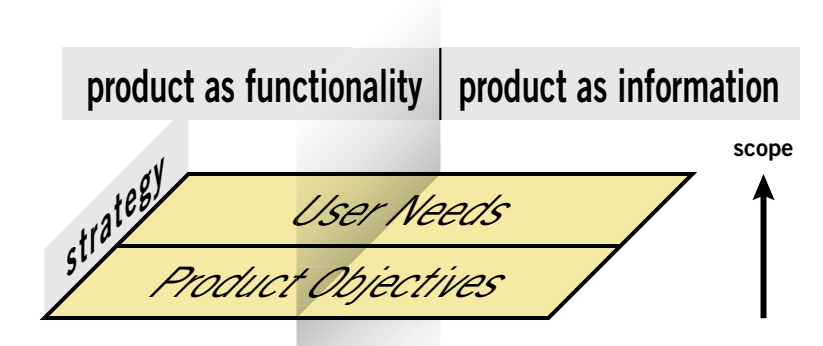
\includegraphics[width=\linewidth]{images/pic2.png}
        \caption{Strategy plane}
    \end{figure}
\section{Product Objectives}
    Is it a service or product? Usually we do not clear our objectives in case of product and thus different people will have different ideas.
\subsection{Business Goals}
    Sometimes you say, ‘To earn money’ or ‘To Save money’. These are too general. On the other hand, very specific, such as ‘To provide text messaging service for users’, which does not explain the requirement of you. We tell the conditions for success, not path.
\subsection{Brand Identity}
    Your brand is neither only a logo nor typography. It can be represented by users’ interaction with your website. This experience would be your brand.
\subsection{Success Metrics}
    You should have some concrete criterias which determines, when you have reached success. These are known as \textbf{success metrics}. These metrics may be :
    \begin{itemize}
        \item The average time, a user spends on the site
        \item Number of visits per registered user
        \item The number of time, each ads is displayed.
        \item The number of calls to support team.
        \item Number of return visits
    \end{itemize}
    Sometimes these metrics are influenced by other factors, For example: Ineffective advertisements. This should be taken into account.
\section{User Needs}
We should not design for ourselves, we should determine the user needs. We should define out users. Ask from users and observe their behaviour.
Prioritize what users need when they use our software.
\subsection{User Segmentation}
Segmentize users into several groups with similar needs. 
They can be grouped by the following characteristics:
\begin{itemize}
    \item gender
    \item averageeducation level
    \item marital status
    \item income
    \item unmarried, college-educated women 25-34 making over \$50000 annually.
\end{itemize}
\begin{figure}
    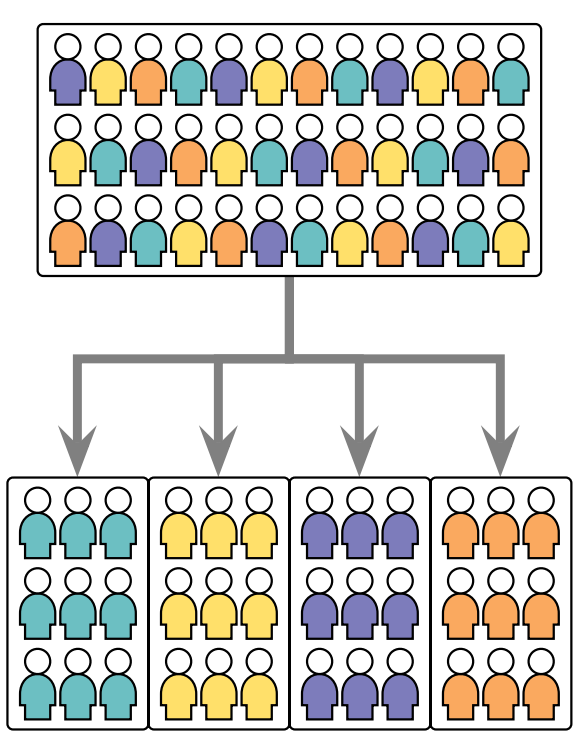
\includegraphics[width=\linewidth]{images/pic3.png}
\end{figure}
\subsection{Usability and User Research}
\textbf{User research} is the process of collecting data to get sense of our users. Some research tools are:
\begin{itemize}
    \item surveys
    \item interviews
    \item user tests
    \item field studies
\end{itemize}
\subsection{Creating Personas}
We formed groups of people but we need more realization, So that It is easier to understand them. For example our site is designed for those who want 
to run their own business. We know that our users fall into the range of 30-45 of age and they are mostly comfortable with web technology. Some of them are 
comfortable with business world while others are newcommers. We can create two persons:
\begin{itemize}
    \item Janet, 42 yo, married and she has two children. she was vice president. frustrated with working for others and wants to start new business
    \item Frank, 37 yo. married and having one child. hobbyist woodworker, Perhaps starting new business will stop her driving job.
\end{itemize}
These two people does not exist but we gave them existance to make them easier to understand following by printing cards with their 
unreal photos and distribute these cards around the office.
\begin{figure}
    \centering
        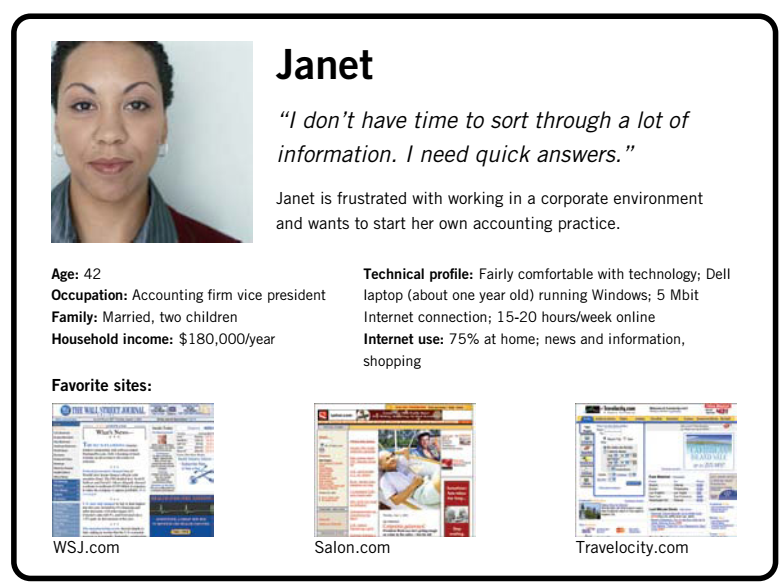
\includegraphics[width=10cm]{images/pic4.png}
    \label{Janet}
\end{figure}
\begin{figure}[]
    \centering
        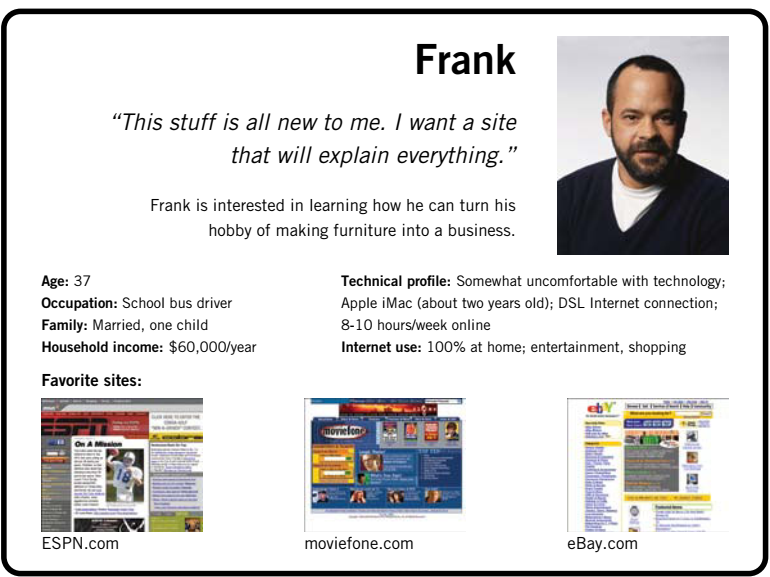
\includegraphics[width=10cm]{images/pic5.png}
    \caption{}
    \label{Frank}
\end{figure}
\section{Team Roles and Process}
